\subsection{Why the operation taxonomy adds little: an information-theoretic account}
\label{sec:rq_why}

Section~\ref{sec:rq_representation} reports that adding $\phi$ to $\kappa$ buys
little, and that $\phi$ alone is weaker than $\kappa$. Two different questions
are involved, and both can be answered exactly, without training anything,
because $\phi$ and $\kappa$ are both functions of the same node. Over every
node of a corpus we compute their joint distribution and two conditional
entropies.
\begin{itemize}
    \item $H(\phi \mid \kappa)$ is the information in the taxonomy that the grammar
          kind does not already supply. If it is near zero, adding $\phi$ to
          $\kappa$ cannot help.
    \item $H(\kappa \mid \phi)$ is the information in the grammar kind that the
          taxonomy destroys. If it is large, $\phi$ alone is a lossy copy of a
          representation that works.
\end{itemize}

% Generated by experiments/emit_tables.py -- DO NOT EDIT BY HAND.
% Every value is read from experiments/results/*.json.

\begin{table}[t]
\centering
\caption{RQ2b: information shared between the operation taxonomy and the
grammar kind, computed exactly over every AST node of the corpora indicated.
Brackets are 95\% bootstrap intervals resampling functions.
$H(\phi \mid \kappa)$ is what the taxonomy adds to the grammar kind, and
$H(\kappa \mid \phi)$ is what the taxonomy throws away.}
\label{tab:rq2b_information}
\resizebox{\linewidth}{!}{%
\begin{tabular}{lrrr}
\toprule
 & BigVul & Devign & DiverseVul \\
\midrule
Sample & 10,000 fn / 918,269 nodes & 10,000 fn / 1,356,164 nodes & 10,000 fn / 1,082,049 nodes \\
\midrule
$H(\phi)$ & 1.449 & 1.504 & 1.477 \\
$H(\kappa)$ & 4.499 & 4.430 & 4.507 \\
\midrule
\multicolumn{4}{l}{\emph{What the taxonomy adds to the grammar kind}} \\
$H(\phi \mid \kappa)$ & \textbf{0.053} $[0.052, 0.054]$ & \textbf{0.060} $[0.060, 0.061]$ & \textbf{0.061} $[0.060, 0.062]$ \\
$I(\phi;\kappa)/H(\phi)$ & 96.3\% & 96.0\% & 95.9\% \\
$\phi$ predictable from $\kappa$ & \textbf{98.4\%} & \textbf{97.7\%} & \textbf{98.0\%} \\
\midrule
\multicolumn{4}{l}{\emph{What the taxonomy discards from the grammar kind}} \\
$H(\kappa \mid \phi)$ & \textbf{3.103} $[3.093, 3.114]$ & \textbf{2.987} $[2.975, 2.998]$ & \textbf{3.091} $[3.080, 3.101]$ \\
$H(\kappa \mid \phi)/H(\kappa)$ & 69.0\% & 67.4\% & 68.6\% \\
\bottomrule
\end{tabular}}
\end{table}


\begin{figure}[t]
\centering
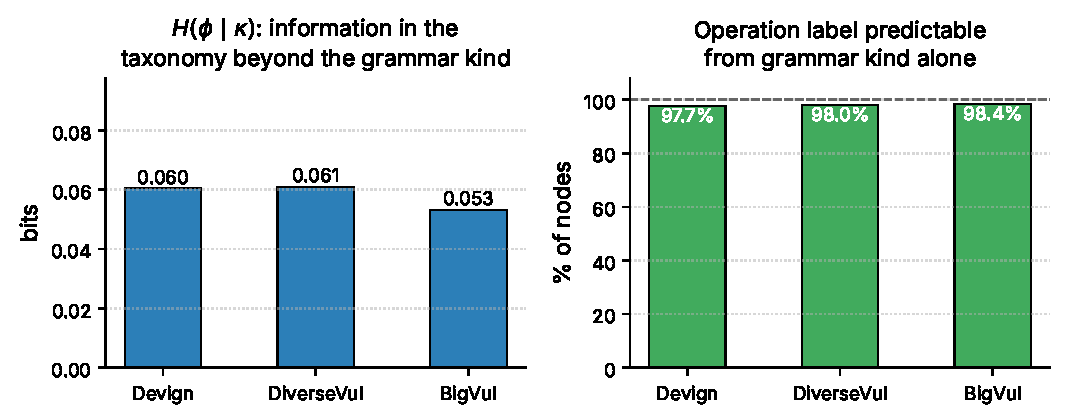
\includegraphics[width=\linewidth]{figures/fig_redundancy.pdf}
\caption{The information the taxonomy carries beyond the grammar kind,
$H(\phi \mid \kappa)$ (left), and the share of nodes whose operation label is
recoverable from the kind alone (right).}
\label{fig:redundancy}
\end{figure}

\textbf{The taxonomy adds almost nothing to the kind.} $H(\phi \mid \kappa)$
lies between \numhPhiGivenKindMin{} and \numhPhiGivenKindMax{} bits on the
three corpora (Table~\ref{tab:rq2b_information}); \numbigvulDeterminism\% of
BigVul nodes have an operation label that is fixed by the node kind. This
follows from the definition rather than from an accident of the data: rules~2
and~3 of Section~\ref{sec:phi} are decided by the node kind or its operator
token, so for most kinds $\phi$ is a constant function of $\kappa$. Only
call expressions (is this callee a memory operation?) and binary expressions
(which operator?) carry residual uncertainty.

\textbf{The taxonomy discards much of the kind.} $H(\kappa \mid \phi)$ is
\numbigvulHKindGivenPhi{} bits on BigVul, \numbigvulKindLost\% of the kind's
entropy: collapsing 364 kinds into nine operation types throws away about two
thirds of what the kind alphabet distinguishes. So $\phi$ is not a neutral
re-encoding of $\kappa$; it is a lossy compression, and an abstraction in that
position cannot be expected to outperform its source.

These are properties of two deterministic labelling functions over a joint
table of $|\mathcal{T}_8| \times |K|$ cells, so they converge quickly: the
bootstrap intervals over functions in Table~\ref{tab:rq2b_information} are
narrower than $0.02$ bits. The diagnostic costs minutes, needs no training, and
would have predicted the experimental pattern of the next sections from the
definition of $\phi$ alone. We offer it as a reusable check for anyone who
proposes an engineered abstraction over a parse tree: compute
$H(\text{abstraction} \mid \text{grammar kind})$ and $H(\text{grammar kind}
\mid \text{abstraction})$ before crediting the abstraction with an effect.
